
\begin{table}
\centering
\begin{tabular}{|l|ll|}
\multicolumn{3}{c}{$\Pr(\ancestralSplitRV=\ancestralSplit_k \mid \siteSplitRV=\siteSplit_j, \tau_1, t)$}\\
\hline
& \multicolumn{2}{|c|}{$\ancestralSplit_k$}\\
    \hline
    $\siteSplit_j$    &$\emptyset$                                &$\{2\}$  \\
    \hline
     $\emptyset$   &$(1+x)^2   (1+w)(1+y)^2$          &$(1+x)^2   (1-w)(1-y)^2$\\
     $\{1\}$       &$(1+x)(1-x)(1+w)(1+y)^2$          &$(1+x)(1-x)(1-w)(1-y)^2$\\
     $\{2\}$       &$(1+x)^2   (1+w)(1+y)(1-y)$       &$(1+x)^2   (1-w)(1+y)(1-y)$\\
     $\{3\}$       &$(1+x)(1-x)(1+w)(1+y)^2$          &$(1+x)(1-x)(1-w)(1-y)^2$\\
     $\{1,2\}$     &$(1+x)(1-x)(1+w)(1+y)(1-y)$       &$(1+x)(1-x)(1-w)(1+y)(1-y)$\\
     $\{1,3\}$     &$(1-x)^2   (1+w)(1+y)^2$          &$(1-x)^2   (1-w)(1-y)^2$\\
     $\{2,3\}$     &$(1+x)(1-x)(1+w)(1+y)(1-y)$       &$(1+x)(1-x)(1-w)(1+y)(1-y)$\\
     $\{1,2,3\}$   &$(1-x)^2   (1+w)(1+y)(1-y)$       &$(1-x)^2   (1-w)(1+y)(1-y)$\\
    \hline
    \hline
    &$\{1\}$                             &$\{1,2\}$  \\
    \hline
     $\emptyset$   &$(1-x)^2   (1-w)(1+y)^2$     &$(1-x)^2   (1+w)(1-y)^2$\\
     $\{1\}$       &$(1+x)(1-x)(1-w)(1+y)^2$     &$(1+x)(1-x)(1+w)(1-y)^2$\\
     $\{2\}$       &$(1-x)^2   (1-w)(1+y)(1-y)$  &$(1-x)^2   (1+w)(1+y)(1-y)$\\
     $\{3\}$       &$(1+x)(1-x)(1-w)(1+y)^2$     &$(1+x)(1-x)(1+w)(1-y)^2$\\
     $\{1,2\}$     &$(1+x)(1-x)(1-w)(1+y)(1-y)$  &$(1+x)(1-x)(1+w)(1+y)(1-y)$\\
     $\{1,3\}$     &$(1+x)^2   (1-w)(1+y)^2$     &$(1+x)^2   (1+w)(1-y)^2$\\
     $\{2,3\}$     &$(1+x)(1-x)(1-w)(1+y)(1-y)$  &$(1+x)(1-x)(1+w)(1+y)(1-y)$\\
     $\{1,2,3\}$   &$(1+x)^2   (1-w)(1+y)(1-y)$  &$(1+x)^2   (1+w)(1+y)(1-y)$\\
    \hline
\end{tabular}
\caption{Likelihood calculations for all site splits $\siteSplit_j$ and ancestral state splits $\ancestralSplit_k$ of the InvFels tree $\tau_1$.
All values multiplied by $1/32$.}
\label{tab:farris_likelihoods}
\end{table}
 
\begin{table}
\centering
\begin{tabular}{|l|ll|}
\multicolumn{3}{c}{$\Pr(\ancestralSplitRV=\ancestralSplit_k \mid \siteSplitRV=\siteSplit_j, \tau_2, t)$}\\
\hline
& \multicolumn{2}{|c|}{$\ancestralSplit_k$}\\
    \hline
    $\siteSplit_j$    &$\emptyset$                                &$\{2\}$  \\
    \hline
     $\emptyset$   &$(1+x)^2   (1+w)(1+y)^2$           &$(1+x)(1-x)(1-w)(1+y)(1-y)$\\
     $\{1\}$       &$(1+x)(1-x)(1+w)(1+y)^2$           &$(1-x)^2   (1-w)(1+y)(1-y)$\\
     $\{2\}$       &$(1+x)^2   (1+w)(1+y)(1-y)$        &$(1+x)(1-x)(1-w)(1-y)^2$\\
     $\{3\}$       &$(1+x)(1-x)(1+w)(1+y)^2$           &$(1+x)^2   (1-w)(1+y)(1-y)$\\
     $\{1,2\}$     &$(1+x)(1-x)(1+w)(1+y)(1-y)$        &$(1-x)^2   (1-w)(1-y)^2$\\
     $\{1,3\}$     &$(1-x)^2   (1+w)(1+y)^2$           &$(1+x)(1-x)(1-w)(1+y)(1-y)$\\
     $\{2,3\}$     &$(1+x)(1-x)(1+w)(1+y)(1-y)$        &$(1+x)^2   (1-w)(1-y)^2$\\
     $\{1,2,3\}$   &$(1-x)^2   (1+w)(1+y)(1-y)$        &$(1+x)(1-x)(1-w)(1-y)^2$\\
    \hline
    \hline
    &$\{1\}$                             &$\{1,2\}$  \\
    \hline
     $\emptyset$   &$(1+x)(1-x)(1-w)(1+y)(1-y)$        &$(1-x)^2   (1+w)(1-y)^2$\\
     $\{1\}$       &$(1+x)^2   (1-w)(1+y)(1-y)$        &$(1+x)(1-x)(1+w)(1-y)^2$\\
     $\{2\}$       &$(1+x)(1-x)(1-w)(1+y)^2$           &$(1-x)^2   (1+w)(1+y)(1-y)$\\
     $\{3\}$       &$(1-x)^2   (1-w)(1+y)(1-y)$        &$(1+x)(1-x)(1+w)(1-y)^2$\\
     $\{1,2\}$     &$(1+x)^2   (1-w)(1+y)^2$           &$(1+x)(1-x)(1+w)(1+y)(1-y)$\\
     $\{1,3\}$     &$(1+x)(1-x)(1-w)(1+y)(1-y)$        &$(1+x)^2   (1+w)(1-y)^2$\\
     $\{2,3\}$     &$(1-x)^2   (1-w)(1+y)^2$           &$(1+x)(1-x)(1+w)(1+y)(1-y)$\\
     $\{1,2,3\}$   &$(1+x)(1-x)(1-w)(1+y)^2$           &$(1+x)^2   (1+w)(1+y)(1-y)$\\
\hline
\end{tabular}
\caption{Likelihood calculations for all site splits $\siteSplit_j$ and ancestral state splits $\ancestralSplit_k$ of the Felsenstein tree $\tau_2$.
All values multiplied by $1/32$.}
\label{tab:fels_likelihoods}
\end{table}
 
\begin{table}
\centering
\begin{tabular}{|l|ll|}
    \multicolumn{3}{c}{InvFels tree ($\tau=\tau_1$)}\\
    \hline
    $\siteSplit_j$    & $\ancestralSplitPartition_j(\tau, t)$ & $\Pr(\ancestralSplitRV=\xi_j \mid \siteSplitRV=\siteSplit_j,\tau,t)$\\
    \hline
    $\emptyset$&
    $\emptyset$&
    $(1+x)^2   (1+w)(1+y)^2$\\
     $\{1\}$    &
    $\emptyset$&
    $(1+x)(1-x)(1+w)(1+y)^2$\\
     $\{2\}$    &
    $\emptyset$&
    $(1+x)^2   (1+w)(1+y)(1-y)$\\
     $\{3\}$    &
    $\emptyset$&
    $(1+x)(1-x)(1+w)(1+y)^2$\\
    $\{1,2\}$  &
    $\{\emptyset,\{1,2\}\}$&
    $(1+x)(1-x)(1+w)(1+y)(1-y)$\\
    $\{1,3\}$  &
    $\left\{\begin{array}{l}
                    \emptyset\\
                    \{1\}\\
                    \{1,2\}
                \end{array}\right.$&
    $\begin{array}{l}
                    (1-x)^2   (1+w)(1+y)^2\\
                    (1+x)^2   (1-w)(1+y)^2\\
                    (1+x)^2   (1+w)(1-y)^2
                \end{array}$\\
    $\{2,3\}$  &
                $\{\emptyset,\{1,2\}\}$&
                $(1+x)(1-x)(1+w)(1+y)(1-y)$\\
    $\{1,2,3\}$&
                $\{1,2\}$&
                $(1+x)^2   (1+w)(1+y)(1-y)$\\
    \hline
    \multicolumn{3}{c}{Felsenstein tree ($\tau=\tau_2$)}\\
    \hline
    $\siteSplit_j$    & $\ancestralSplitPartition_j(\tau, t)$ & $\Pr(\ancestralSplitRV=\xi_j \mid \siteSplitRV=\siteSplit_j,\tau,t)$\\
    \hline
    $\emptyset$       &$\emptyset$&$(1+x)^2   (1+w)(1+y)^2$\\
    $\{1\}$          &
    $\left\{\begin{array}{l}
                    \emptyset\\
                    \{1\}
                \end{array}\right.$&
    $\begin{array}{l}
                        (1+x)(1-x)(1+w)(1+y)^2\\
                        (1+x)^2   (1-w)(1+y)(1-y)
                    \end{array}$\\
      $\{2\}$          &
    $\left\{\begin{array}{l}
                    \emptyset\\
                    \{1\}
                \end{array}\right.$&
    $\begin{array}{l}
                    (1+x)^2   (1+w)(1+y)(1-y)\\
                    (1+x)(1-x)(1-w)(1+y)^2
                    \end{array}$\\
      $\{3\}$          &
    $\left\{\begin{array}{l}
                    \emptyset\\
                    \{2\}
                \end{array}\right.$&
    $\begin{array}{l}
                    (1+x)(1-x)(1+w)(1+y)^2\\
                    (1+x)^2   (1-w)(1+y)(1-y)
                    \end{array}$\\
     $\{1,2\}$         &
    $\left\{\begin{array}{l}
                    \{\emptyset,\{1,2\}\}\\
                    \{1\}
                \end{array}\right.$&
    $\begin{array}{l}
                    (1+x)(1-x)(1+w)(1+y)(1-y)\\
                    (1+x)^2   (1-w)(1+y)^2
                    \end{array}$\\
     $\{1,3\}$         &
    $\left\{\begin{array}{l}
                    \emptyset\\
                    \{\{1\},\{2\}\}\\
                    \{1,2\}
                \end{array}\right.$&
    $\begin{array}{l}
                    (1-x)^2   (1+w)(1+y)^2\\
                    (1+x)(1-x)(1-w)(1+y)(1-y)\\
                    (1+x)^2   (1+w)(1-y)^2
                    \end{array}$\\
      $\{2,3\}$        &
    $\left\{\begin{array}{l}
                    \{\emptyset,\{1,2\}\}\\
                    \{1\}\\
                    \{2\}
                \end{array}\right.$&
    $\begin{array}{l}
                    (1+x)(1-x)(1+w)(1+y)(1-y)\\
                    (1-x)^2   (1-w)(1+y)^2\\
                    (1+x)^2   (1-w)(1-y)^2
                    \end{array}$\\
     $\{1,2,3\}$       &
    $\left\{\begin{array}{l}
                    \{2\} \\
                    \{1,2\}
                \end{array}\right.$&
    $\begin{array}{l}
                    (1+x)(1-x)(1-w)(1+y)^2 \\
                    (1+x)^2   (1+w)(1+y)(1-y)
                    \end{array}$\\
    \hline
\end{tabular}
\caption{Likelihood calculations for all site splits $\siteSplit_j$ and ancestral state partitions $\ancestralSplitPartition_j$ after maximizing over ancestral states on the InvFels tree $\tau_1$ and the Felsenstein tree $\tau_2$.
All values multiplied by $1/32$.
Likelihoods with multiple entries have maxima determined by unknown branch length parameters.
See Tables~\ref{tab:farris_likelihoods} and~\ref{tab:fels_likelihoods} for full calculations.}
\label{tab:likelihoods}
\end{table}

\topoInconsist*

\begin{proof}
Assume $\tau^*=\tau_1$.
The InvFels tree log-likelihood takes one of three values depending on branch lengths, which is due to site split $\{1,3\}$ (see the upper table of Table~\ref{tab:likelihoods}).

We write out the case for the ancestral state split $\{1\}$, and show the other two cases follow a similar argument.
Directly substituting calculations from Table~\ref{tab:sitepatprob} and Table~\ref{tab:likelihoods} where $\tau = \tau_1$ in \eqref{eq:site_pattern_profile_likelihood_mean}, the log-likelihood is, suppressing normalizing constants $-\log 8$ (from the first additive term of \eqref{eq:site_pattern_profile_likelihood_mean}) and $-\log 32$ (from the second),
\begin{align}
    \label{eq:farris_likelihood}
    \ell_{\tau_1,t^*}(\tau_1, t)
    &=        p_{\emptyset}  \cdot\log(1+x^2+y^2+4xyw+x^2y^2) \nonumber \\
    &\qquad + p_{1}          \cdot\log(1-x^2+y^2-x^2y^2) \nonumber \\
    &\qquad + p_{2}          \cdot\log(1+x^2-y^2-x^2y^2) \nonumber \\
    &\qquad + p_{3}          \cdot\log(1-x^2+y^2-x^2y^2) \nonumber \\
    &\qquad + p_{12}         \cdot\log(1-x^2-y^2+x^2y^2) \nonumber \\
    &\qquad + p_{13}         \cdot\log(1+x^2+y^2-4xyw+x^2y^2) \nonumber \\
    &\qquad + p_{23}         \cdot\log(1-x^2-y^2+x^2y^2) \nonumber \\
    &\qquad + p_{123}        \cdot\log(1+x^2-y^2-x^2y^2) \nonumber \\
    &\qquad + p_{\emptyset}  \cdot\log((1+x)^2   (1+w)(1+y)^2) \nonumber \\
    &\qquad + p_{1}          \cdot\log((1+x)(1-x)(1+w)(1+y)^2) \nonumber \\
    &\qquad + p_{2}          \cdot\log((1+x)^2   (1+w)(1+y)(1-y)) \nonumber \\
    &\qquad + p_{3}          \cdot\log((1+x)(1-x)(1+w)(1+y)^2) \nonumber \\
    &\qquad + p_{12}         \cdot\log((1+x)(1-x)(1+w)(1+y)(1-y)) \nonumber \\
    &\qquad + p_{13}         \cdot\log((1+x)^2   (1-w)(1+y)^2) \nonumber \\
    &\qquad + p_{23}         \cdot\log((1+x)(1-x)(1+w)(1+y)(1-y)) \nonumber \\
    &\qquad + p_{123}        \cdot\log((1+x)^2   (1+w)(1+y)(1-y)).
\end{align}
Our plan is to simplify the likelihood to remove log-of-quadratic terms of $x,y,$ and $w$, obtaining an upper bound on the likelihood that has a closed-form maximum in each variable.
To bound the generating probabilities, we use the facts that, for $x,y\in[0,1]$,
\begin{align*}
p_{12} = p_{23} \propto 1-x^2-y^2+x^2y^2 & = (1+x)(1-x)(1+y)(1-y) \\
p_{1} = p_{3} \propto 1-x^2+y^2-x^2y^2 & = (1+x)(1-x)(1+y^2) \le (1+x)(1-x)(1+y) \\
p_{2} = p_{123} \propto 1+x^2-y^2-x^2y^2 & = (1+x^2)(1+y)(1-y) \le (1+x)(1+y)(1-y).
\end{align*}
To bound the remaining $p_{\emptyset}$ and $p_{13}$, we use
\begin{align*}
1+x^2+y^2+x^2y^2 & = (1+x^2)(1+y^2) \le (1+x)(1+y) \\
4xy & = 2x \cdot 2y \le (1+x^2)(1+y^2) \le (1+x)(1+y)
\end{align*}
so that the $p_{\emptyset}$ term is bounded as
\begin{align*}
    p_{\emptyset} & \propto 1+x^2+y^2+4xyw+x^2y^2 \\
                  & \le 1+x^2+y^2+4xy+x^2y^2 \\
                  & \le 2(1+x)(1+y)
\end{align*}
and $p_{13}$ is bounded as
\begin{align*}
    p_{13} & \propto 1+x^2+y^2-4xyw+x^2y^2 \\
                  & \le 1+x^2+y^2+x^2y^2 \\
                  & \le (1+x)(1+y).
\end{align*}
Factoring and making these substitutions (again, under the assumption that the ancestral state split is $\{1\}$) results in
\begin{align*}
&    \ell_{\tau_1,t^*}(\tau_1, t) \\
&\qquad \le      p_{\emptyset}  \cdot\log(2(1+x)(1+y))
+ p_{1}          \cdot\log((1+x)(1-x)(1+y)) \\
    &\qquad\qquad + p_{2}          \cdot\log((1+x)(1+y)(1-y))
+ p_{3}          \cdot\log((1+x)(1-x)(1+y)) \\
    &\qquad\qquad + p_{12}         \cdot\log((1+x)(1-x)(1+y)(1-y))
+ p_{13}         \cdot\log((1+x)(1+y)) \\
    &\qquad\qquad + p_{23}         \cdot\log((1+x)(1-x)(1+y)(1-y))
+ p_{123}        \cdot\log((1+x)(1+y)(1-y)) \\
    &\qquad\qquad + p_{\emptyset}  \cdot\log((1+x)^2   (1+w)(1+y)^2)
+ p_{1}          \cdot\log((1+x)(1-x)(1+w)(1+y)^2) \\
    &\qquad\qquad + p_{2}          \cdot\log((1+x)^2   (1+w)(1+y)(1-y))
+ p_{3}          \cdot\log((1+x)(1-x)(1+w)(1+y)^2) \\
    &\qquad\qquad + p_{12}         \cdot\log((1+x)(1-x)(1+w)(1+y)(1-y))
+ p_{13}         \cdot\log((1+x)^2   (1-w)(1+y)^2) \\
    &\qquad\qquad + p_{23}         \cdot\log((1+x)(1-x)(1+w)(1+y)(1-y)) \\
    &\qquad\qquad + p_{123}        \cdot\log((1+x)^2   (1+w)(1+y)(1-y)) \\
&\qquad =      p_{\emptyset}  \cdot\log(2)
+ \log(1+x)
+ (p_{1}+p_{3}+p_{12}+p_{23})\cdot\log(1-x) \\
&\qquad\qquad + \log(1+y)
+ (p_{2}+p_{12}+p_{23}+p_{123})\cdot\log(1-y) \\
&\qquad\qquad + (2-p_{1}-p_{3}-p_{12}-p_{23})\cdot\log(1+x)
+ (p_{1}+p_{3}+p_{12}+p_{23})\cdot\log(1-x) \\
&\qquad\qquad + (2-p_{2}-p_{12}-p_{23}-p_{123})\cdot\log(1+y)
+ (p_{2}+p_{12}+p_{23}+p_{123})\cdot\log(1-y) \\
&\qquad\qquad + (1-p_{13})\cdot\log(1+w)
+ p_{13}\cdot\log(1-w) \\
&\qquad =      p_{\emptyset}  \cdot\log(2)
+ (3-p_{1}-p_{3}-p_{12}-p_{23})\cdot\log(1+x)
+ 2(p_{1}+p_{3}+p_{12}+p_{23})\cdot\log(1-x) \\
&\qquad\qquad + (3-p_{2}-p_{12}-p_{23}-p_{123})\cdot\log(1+y)
+ 2(p_{2}+p_{12}+p_{23}+p_{123})\cdot\log(1-y) \\
&\qquad\qquad + (1-p_{13})\cdot\log(1+w)
+ p_{13}\cdot\log(1-w).
\end{align*}
To simplify, let
\begin{equation}
    \begin{aligned}
        a_{1} &= 3-p_{1}-p_{3}-p_{12}-p_{23}, \\
        a_{2} &= 2(p_{1}+p_{3}+p_{12}+p_{23}), \\
        a_{3} &= 3-p_{2}-p_{12}-p_{23}-p_{123}, \\
        a_{4} &= 2(p_{2}+p_{12}+p_{23}+p_{123}), \\
    \end{aligned}
    \label{eq:a_const}
\end{equation}
so that
\begin{equation*}
\begin{split}
&    \ell_{\tau_1,t^*}(\tau_1, t) \\
&\qquad \le      p_{\emptyset}  \cdot\log(2)
+ a_{1}\cdot\log(1+x)
+ a_{2}\cdot\log(1-x)
+ a_{3}\cdot\log(1+y) \\
&\qquad\qquad + a_{4}\cdot\log(1-y)
+ (1-p_{13})\cdot\log(1+w)
+ p_{13}\cdot\log(1-w).
\end{split}
\end{equation*}
Maximizing over the unknown terms yields
\[
\hat{x} = \frac{a_{1}-a_{2}}{a_{1}+a_{2}}, \ \hat{y} = \frac{a_{3}-a_{4}}{a_{3}+a_{4}}, \ \hat{w} = 1-2p_{13}.
\]
Trivially $0 \le \hat{w} \le 1$ and $\hat{x}, \hat{y} \le 1$.
We check that $\hat{x}, \hat{y} \ge 0$ to ensure these maxima are valid.
For $\hat{x} \ge 0$ we need $a_1 \ge a_2$; letting
\[
\tilde{p} = p_{1}+p_{3}+p_{12}+p_{23}
\]
we have from \eqref{eq:a_const} that $a_1 \ge a_2$ only if $3 \ge 3\tilde{p}$.
Since $\tilde{p} = 1/8\cdot(4-4(x^*)^2)$, we have $0 \le \tilde{p} \le 1/2$ implying $\hat{x} \ge 0$.
The same approach works for $\hat{y}$.
The upper bound for the likelihood is then maximized at
\begin{align}
\begin{split}
&    \ell_{\tau_1,t^*}(\tau_1, t) \\
&\qquad\le      p_{\emptyset}  \cdot\log(2)
+ a_{1}\cdot\log\frac{2a_{1}}{a_{1}+a_{2}}
+ a_{2}\cdot\log\frac{2a_{2}}{a_{1}+a_{2}}
+ a_{3}\cdot\log\frac{2a_{3}}{a_{3}+a_{4}} \\
&\qquad\qquad + a_{4}\cdot\log\frac{2a_{4}}{a_{3}+a_{4}}
+ (1-p_{13})\cdot\log(2(1-p_{13}))
+ p_{13}\cdot\log(2p_{13}) \\
&\qquad := C^{\{1\}}_{\tau_1,\tau_1}(x^*, y^*).
\end{split}
\label{eq:farris-upper-bound-1}
\end{align}

The other two possible ancestral state splits for the likelihood of the site split $\{1,3\}$ admit similar simplifications, as we now describe.
The upper bound $C^{\{1\}}_{\tau_1,\tau_1}(x^*, y^*)$ in \eqref{eq:farris-upper-bound-1} is for the ancestral state split $\{1\}$.
For the ancestral state split $\emptyset$ we can derive an upper bound $C^{\emptyset}_{\tau_1,\tau_1}(x^*, y^*)$ in \eqref{eq:farris-upper-bound-empty} in a similar fashion, and $C^{\emptyset}_{\tau_1,\tau_1}(x^*, y^*)$ will be the same as $C^{\{1\}}_{\tau_1,\tau_1}(x^*, y^*)$ except we lose a $(1+x)^2$ term, gain a $(1-x)^2$ term, lose a $(1-w)$ term, and gain a $(1+w)$ term.
In this case, all terms involving $w$ simplify to $\log(1+w)$, which is maximized at $\hat{w}=1$.
For the constants above, $a_{1}$ is the multiplier for the $\log(1+x)$ term and $a_{2}$ for the $\log(1-x)$ term meaning that exchanging the above quadratic $x$ terms yields new constants
\begin{equation}
    \begin{aligned}
        a_{1}' &= a_{1}-2p_{13}, \\
        a_{2}' &= a_{2}+2p_{13}, \\
    \end{aligned}
    \label{eq:a_const_prime_x}
\end{equation}
for ancestral state split $\ancestralSplitPartition_j(\tau_1, t) = \emptyset$, yielding the upper bound
\begin{align}
\begin{split}
&    \ell_{\tau_1,t^*}(\tau_1, t) \\
&\qquad\le      p_{\emptyset}  \cdot\log(2)
+ a_{1}'\cdot\log\frac{2a_{1}'}{a_{1}'+a_{2}'}
+ a_{2}'\cdot\log\frac{2a_{2}'}{a_{1}'+a_{2}'} \\
&\qquad\qquad + a_{3}\cdot\log\frac{2a_{3}}{a_{3}+a_{4}}
+ a_{4}\cdot\log\frac{2a_{4}}{a_{3}+a_{4}}
+ \log(2) \\
&\qquad := C^{\emptyset}_{\tau_1,\tau_1}(x^*, y^*).
\end{split}
\label{eq:farris-upper-bound-empty}
\end{align}

For ancestral state split $\ancestralSplitPartition_j(\tau_1, t) = \{1,2\}$, we have constants
\begin{equation}
    \begin{aligned}
        a_{3}' &= a_{3}-2p_{13}, \\
        a_{4}' &= a_{4}+2p_{13}, \\
    \end{aligned}
    \label{eq:a_const_prime_y}
\end{equation}
and the upper bound
\begin{align}
\begin{split}
&    \ell_{\tau_1,t^*}(\tau_1, t) \\
&\qquad\le      p_{\emptyset}  \cdot\log(2)
+ a_{1}\cdot\log\frac{2a_{1}}{a_{1}+a_{2}}
+ a_{2}\cdot\log\frac{2a_{2}}{a_{1}+a_{2}} \\
&\qquad\qquad+ a_{3}'\cdot\log\frac{2a_{3}'}{a_{3}'+a_{4}'}
+ a_{4}'\cdot\log\frac{2a_{4}'}{a_{3}'+a_{4}'}
+ \log(2) \\
&\qquad := C^{\{1,2\}}_{\tau_1,\tau_1}(x^*, y^*).
\end{split}
\label{eq:farris-upper-bound-12}
\end{align}

We now need to check that
\[
\hat{x} = \frac{a_{1}'-a_{2}'}{a_{1}'+a_{2}'}, \ \hat{y} = \frac{a_{3}'-a_{4}'}{a_{3}'+a_{4}'}
\]
are both between zero and one.
Using a similar argument as that where $\ancestralSplitPartition_j(\tau_1, t) = \{1\}$, we only need to show $a_1' \ge a_2'$, which is true if $3-2p_{13} \ge 3\tilde{p}+2p_{13}$.
Some rearranging and the fact that $0 \le \tilde{p} \le 1/2$ shows this is equivalent to showing $p_{13} \le 3/8$.
Using Table~\ref{tab:sitepatprob} while setting $t=t^*=\{x^*,y^*,x^*,y^*,y^*\}$,
\[
p_{13} = \frac{1}{8}\left(1 + (x^*)^2 + (y^*)^2 - 4x^*(y^*)^2 + (x^*)^2(y^*)^2\right),
\]
meaning we are interested in whether
\begin{equation}
1 + (x^*)^2 + (y^*)^2 - 4x^*(y^*)^2 + (x^*)^2(y^*)^2 \le 3.
\label{eq:generating_ineq}
\end{equation}
We see that
\begin{equation}
\begin{split}
& 1 + (x^*)^2 + (y^*)^2 - 4x^*(y^*)^2 + (x^*)^2(y^*)^2 \le 3 \\
& \qquad \qquad \qquad \qquad \iff (y^*)^2\left(1 - 4x^* + (x^*)^2\right) \le 2 - (x^*)^2
\end{split}
\label{eq:lenny}
\end{equation}
and that
\begin{align*}
(y^*)^2\left(1 - 4x^* + (x^*)^2\right) &\le (y^*)^2\left(1 - 2x^* + (x^*)^2\right) \\
                                       &=   (y^*)^2\left(1 - x^*\right)^2 \\
                                       &\le        \left(1 - x^*\right)^2 \\
                                       &\le              2 - (x^*)^2,
\end{align*}
with the last inequality holding if $0 \le x^* \le 1$, showing that \eqref{eq:lenny} holds.
Thus, $p_{13} \le 3/8$ and our $\hat{x}$ and $\hat{y}$ are valid.

All bounds are functions only of $x,y$ through the true generating probabilities $x^*, y^*$.
Call the upper bound
\[
C_0(x^*, y^*) := \max\left(C^{\{1\}}_{\tau_1,\tau_1}(x^*, y^*), C^{\emptyset}_{\tau_1,\tau_1}(x^*, y^*), C^{\{1,2\}}_{\tau_1,\tau_1}(x^*, y^*)\right).
\]

We next construct a lower bound on the Felsenstein tree partial likelihood.
In general, taking
\[
\hat{t} = \argmax_{t} \ \tilde{\ell}_{\tau^*,t^*}(\tau, t).
\]
we see
\[
\max_{t} \ \ell_{\tau^*,t^*}(\tau, t) \ge
    \shannonDivergence_{\tau^*,t^*}(\tau,\hat{t})
    + \tilde{\ell}_{\tau^*,t^*}(\tau, \hat{t})
\]
is a lower bound for the joint maximum of \eqref{eq:log_likelihood_simplified}.
In the Felsenstein case, there are many more optimal internal states depending on branch lengths than in the InvFels case (see the lower table of Table~\ref{tab:likelihoods}).
We first bound the entire likelihood below and then proceed with joint inference.
To obtain a lower bound for the likelihood we replace $1+w$ with $1-w$ in Table~\ref{tab:likelihoods} for $\tau = \tau_2$; in this case, we resolve many of the ambiguous likelihood terms.
For example, for site split $\{1,2\}$, after we replace the $1+w$ term for $\ancestralSplitPartition_j(\tau, t)=\{\emptyset, \{1,2\}\}$ with $1-w$, we have
\[
\max\left((1+x)^2 (1-w)(1+y)^2, (1+x)(1-x)(1-w)(1+y)(1-y)\right)
\]
where since
\[
(1+x)^2 (1-w)(1+y)^2 > (1+x)(1-x)(1-w)(1+y)(1-y),
\]
the maximum for this site split can be bounded below by $(1+x)^2 (1-w)(1+y)^2$.
For the other site splits we consider three cases.
If $(1+x)(1-y) > (1-x)(1+y)$, then
\[
(1+x)^2(1-w)(1+y)(1-y) > (1+x)(1-x)(1-w)(1+y)^2
\]
meaning the cases $\{1\}, \{2\}, \{3\}$ and $\{1,2,3\}$ will have likelihoods bounded below by
\[
(1+x)^2(1-w)(1+y)(1-y).
\]
For the cases $\{1,3\}$ and $\{2,3\}$ and the same condition, we have
\[
(1+x)^2(1-w)(1-y)^2 > (1-x)^2(1-w)(1+y)^2
\]
and
\[
(1+x)^2(1-w)(1-y)^2 > (1+x)(1-x)(1-w)(1+y)(1-y),
\]
yielding lower bounds of
\[
(1+x)^2(1-w)(1-y)^2
\]
in these cases.
The partial likelihood in this case is then bounded below by
\begin{align*}
    \tilde{\ell}_{\tau_1,t^*}(\tau_2, t)
    &\ge      p_{\emptyset}  \cdot\log((1+x)^2   (1-w)(1+y)^2) \\
    &\qquad + p_{1}          \cdot\log((1+x)^2   (1-w)(1+y)(1-y)) \\
    &\qquad + p_{2}          \cdot\log((1+x)^2   (1-w)(1+y)(1-y)) \\
    &\qquad + p_{3}          \cdot\log((1+x)^2   (1-w)(1+y)(1-y)) \\
    &\qquad + p_{12}         \cdot\log((1+x)^2   (1-w)(1+y)^2) \\
    &\qquad + p_{123}        \cdot\log((1+x)^2   (1-w)(1+y)(1-y))\\
    &\qquad + p_{13}         \cdot\log((1+x)^2   (1-w)(1-y)^2) \\
    &\qquad + p_{23}         \cdot\log((1+x)^2   (1-w)(1-y)^2).
\end{align*}
When $(1+x)(1-y) < (1-x)(1+y)$, similar arguments yield the lower bound
\begin{align*}
    \tilde{\ell}_{\tau_1,t^*}(\tau_2, t)
    &\ge      p_{\emptyset}  \cdot\log((1+x)^2    (1-w)(1+y)^2) \\
    &\qquad + p_{1}          \cdot\log((1+x)(1-x)(1-w)(1+y)^2) \\
    &\qquad + p_{2}          \cdot\log((1+x)(1-x)(1-w)(1+y)^2) \\
    &\qquad + p_{3}          \cdot\log((1+x)(1-x)(1-w)(1+y)^2) \\
    %See above.
    &\qquad + p_{12}         \cdot\log((1+x)^2    (1-w)(1+y)^2) \\
    &\qquad + p_{123}        \cdot\log((1+x)(1-x)(1-w)(1+y)^2)\\
    &\qquad + p_{13}         \cdot\log((1-x)^2    (1-w)(1+y)^2) \\
    &\qquad + p_{23}         \cdot\log((1-x)^2    (1-w)(1+y)^2).
\end{align*}
Finally, if $(1+x)(1-y) = (1-x)(1+y)$, $x=y$ and the lower bound will be less than the other cases.
Letting
\[
b = p_{1}+p_{2}+p_{3}+p_{123}
\]
yields
\[
    \tilde{\ell}_{\tau_1,t^*}(\tau_2, t)
    \ge      2\cdot\log(1+x)
    + (2-b)  \cdot\log(1+y)
    + b      \cdot\log(1-y)
    + \log(1-w)
\]
for the first lower bound, and we get the equivalent expression for the second lower bound by exchanging $x$ and $y$.
Moreover, the divergence quanitity is unchanged when exchanging $x$ and $y$ provided $w=0$.
Maximizing either lower bound over $t$, we obtain
\[
\tilde{\ell}_{\tau_1,t^*}(\tau_2, t)
\ge      2\cdot\log(2)
+ (2-b)  \cdot\log(2-b)
+ b      \cdot\log(b),
\]
i.e., the maximum is achieved at $\{1,1-b,0\}$.
Our lower bound is
\[
C_1(x^*, y^*) := \shannonDivergence_{\tau_1,t^*}(\tau_2,\{1,1-b,0\}) + 2\cdot\log(2) + (2-b)\cdot\log(2-b) + b\cdot\log(b).
\]
See Fig.~\ref{fig:inconsistency-farris} for the values of $0 < p_{x^*}, p_{y^*} < 1$ with $p_{x^*}=(1-x^*)/2$ and $p_{y^*}=(1-y^*)/2$ where $C_1(x^*, y^*) > C_0(x^*, y^*)$ and joint inference is inconsistent.
\end{proof}

\generalBranchInconsist*

\begin{proof}
Recalling Table~\ref{tab:likelihoods} for the InvFels tree $\tau = \tau_1$, the likelihood can take one of three forms corresponding to which ancestral state for $\siteSplit_j=\{1,3\}$ maximizes the likelihood over $(x,y,w)$.
In general, $\hat{w}$ is a function of $x^*$, $y^*$, $\hat{x}$, and $\hat{y}$.
Assume we know $\hat{x}$ and $\hat{y}$ as functions of $x^*$ and $y^*$ only.
By collapsing like terms and ignoring terms without $w$, the log-likelihood in \eqref{eq:farris_likelihood} as a function of $w$ is
\begin{align*}
    \ell_{\tau_1,t^*}(\tau_1, w)
    &\sim     p_{\emptyset}  \cdot\log(1+(\hat{x})^2+(\hat{y})^2+4\hat{x}\hat{y}w+(\hat{x})^2(\hat{y})^2) \\
    &\qquad + p_{13}         \cdot\log(1+(\hat{x})^2+(\hat{y})^2-4\hat{x}\hat{y}w+(\hat{x})^2(\hat{y})^2) \\
    &\qquad + (1 - p_{13})\cdot\log(1+w) \\
    &\qquad + p_{13}\cdot\log(1-w)
\end{align*}
where $\sim$ denotes equality up to an additive constant.
Similarly, the other two possibilities for the likelihood both satisfy
\begin{align*}
    \ell_{\tau_1,t^*}(\tau_1, w)
    &\sim     p_{\emptyset}  \cdot\log(1+(\hat{x})^2+(\hat{y})^2+4\hat{x}\hat{y}w+(\hat{x})^2(\hat{y})^2) \\
    &\qquad + p_{13}         \cdot\log(1+(\hat{x})^2+(\hat{y})^2-4\hat{x}\hat{y}w+(\hat{x})^2(\hat{y})^2) \\
    &\qquad + \log(1+w).
\end{align*}
Since
\[
\log(1+w) \geq (1 - p_{13})\cdot\log(1+w) + p_{13}\cdot\log(1-w)
\]
with equality only when $w=0$, the second likelihood is the likelihood with the maximum-likelihood ancestral state, and so we only analyze that case.

Now substitute in values for $p_{\emptyset}$ and $p_{13}$ from Table~\ref{tab:sitepatprob}.
Simplifying, the likelihood can be written
\[
\ell(w) = \alpha_1\log(\beta+\gamma w) + \alpha_2\log(\beta-\gamma w) + \log(1+w)
\]
where
\[
\alpha_1 := \alpha_1(x^*, y^*) = \frac{1}{8} \left(1+(x^*)^2+(y^*)^2+4x^*(y^*)^2+(x^*)^2(y^*)^2\right),
\]
\[
\alpha_2 := \alpha_2(x^*, y^*) = \frac{1}{8}\left(1+(x^*)^2+(y^*)^2-4x^*(y^*)^2+(x^*)^2(y^*)^2\right),
\]
\[
\beta := \beta(\hat{x}, \hat{y}) = 1+(\hat{x})^2+(\hat{y})^2+(\hat{x})^2(\hat{y})^2,
\]
\[
\gamma := \gamma(\hat{x}, \hat{y}) = 4\hat{x}\hat{y}.
\]
%das: added as assumption to theorem
Since $x^*,y^*,\hat{x},$ and $\hat{y}$ all fall between zero and one, we make use of the inequalities
\[
\alpha_1 > \alpha_2
\]
and
\[
\beta > \gamma
\]
using the assumptions that $x^*=y^*=0$, $\hat{x}=\hat{y}=0$, and $\hat{x}=\hat{y}=1$.
% Not sure if I need to show this, but if x and y aren't 1 it's 1+x^2+y^2+x^2y^2 > 4xy => (1+x^2)(1+y^2) > 4xy and 1+x^2 > 2x, 1+y^2 > 2y qed
The derivative of the log-likelihood with respect to $w$ is
\[
\ell'(w) := \frac{d}{dw} \ell(w) = \frac{\alpha_1 \gamma}{\beta+\gamma w} - \frac{\alpha_2 \gamma}{\beta-\gamma w} + \frac{1}{1+w}.
\]
The inequality $\beta > \gamma$ implies that this function stays finite and that, when considering $\ell'(w) \lessgtr 0$, we equivalently consider $f(w) \lessgtr 0$ where $f$ is the quadratic function
\begin{align*}
f(w) &= (w)^2\cdot(-\gamma^2\alpha_1-\gamma^2\alpha_2-\gamma^2) \\
      &\qquad + w\cdot(\gamma\alpha_1\beta-\gamma^2\alpha_1-\gamma\alpha_2\beta-\gamma^2\alpha_2) \\
      &\qquad + (\gamma\alpha_1\beta-\gamma\alpha_2\beta+\beta^2).
\end{align*}
% Note from das: b^2 - 4ac is always \ge 0 by \alpha_1 > \alpha_2, so b^2 - 4ac can only be zero if b is zero and a or c is zero. c is never zero, so this means a must be zero for this to happen, which only occurs if \gamma = 0, i.e., if x or y is zero.
Using the assumption that $\hat{x}\neq 0$ and $\hat{y}\neq 0$, this implies $\ell'$ has two zeros according to the quadratic formula.
Because $\alpha_1 > \alpha_2$ we have $\ell'(0) > 0$, and thus $\ell$ is increasing at $w=0$.
This implies that if the smaller of the zeros of $f(w)$ is greater than one, then $\hat{w} \equiv 1$.
Using the quadratic formula with
\[
a = -\gamma^2 \alpha_1 - \gamma^2 \alpha_2 - \gamma^2,
\]
\[
b = \gamma \alpha_1 \beta - \gamma^2\alpha_1 - \gamma \alpha_2 \beta - \gamma^2 \alpha_2,
\]
\[
c = \gamma \alpha_1 \beta - \gamma \alpha_2 \beta + \beta^2,
\]
the smaller zero is
\[
\hat{w} = \frac{-b - \sqrt{b^2 - 4ac}}{2a},
\]
which is a function of the generating parameters $x^*$ and $y^*$.
We see that $a \le 0$ and, by a small calculation, $2a+b \leq 0$.
With this we have,
\[
\hat{w} \ge 1 \iff
|2a + b| \leq \sqrt{b^2 - 4ac} \iff
%-b - \sqrt{b^2 - 4ac} \le 2a,
%0 \ge -b - 2a \le \sqrt{b^2 - 4ac},
%b^2 + 4ab + 4a^2 \le b^2 - 4ac,
%a^2 + ab + ac \le 0,
a + b + c \ge 0.
\]
Using
\[
\alpha_1 + \alpha_2 = \frac{1}{4}\left(1+(x^*)^2+(y^*)^2+(x^*)^2(y^*)^2\right)
\]
and
\[
\alpha_1 - \alpha_2 = x^*(y^*)^2,
\]
and simplifying as functions of $\gamma$ and $\beta$ shows that $a + b + c \ge 0$ is equivalent to
\[
-\gamma^2\left(1 + \frac{1}{2}\left(1+(x^*)^2+(y^*)^2+(x^*)^2(y^*)^2\right)\right) + 2\gamma\beta x^*(y^*)^2 + \beta^2 \ge 0,
\]
which, writing out $\gamma$ and $\beta$ explicitly yields
\begin{equation}
\label{eq:general-bl-result}
-\gamma^2(\hat{x}, \hat{y})\left(1 + \frac{1}{2}\left(1+(x^*)^2+(y^*)^2+(x^*)^2(y^*)^2\right)\right) + 2\gamma(\hat{x}, \hat{y})\beta(\hat{x}, \hat{y})x^*(y^*)^2 + \beta^2(\hat{x}, \hat{y}) \ge 0.
\end{equation}
Given the bounds
\[
\gamma_{L} \le \gamma(\hat{x}, \hat{y}) \le \gamma_{U}
\]
and
\[
\beta_{L} \le \beta(\hat{x}, \hat{y}),
\]
if
\[
-\gamma_{U}^2\left(1 + \frac{1}{2}\left(1+(x^*)^2+(y^*)^2+(x^*)^2(y^*)^2\right)\right) + 2\gamma_{L}\beta_{L}x^*(y^*)^2 + \beta_{L}^2 \ge 0,
\]
then \eqref{eq:general-bl-result} holds, and this is an inequality involving only $x^*$ and $y^*$.
\end{proof}
To get a sense of the region of overestimation, Fig.~\ref{fig:bl-loose-inconsistency} plots an intermediate case.

\subsubsection*{Restricted case}

Theorem~\ref{thm:general-bl} allows us to see where inconsistency in branch length estimation arises when performing general joint maximization over all of the branch parameters, though its conclusion is a statement about both the inconsistency of the internal branch estimate as well as about poor estimation of the other branch parameter estimates.
To obtain an analytic result indicating where only the internal branch parameter is inconsistently estimated, we consider a restricted case of Theorem~\ref{thm:general-bl}.
Fix estimated fidelities $x=x^*$ and $y=y^*$ to their true, generating values and estimate the internal branch parameter $w$.
Let
\[
\beta := \beta(x^*, y^*) = 1+(x^*)^2+(y^*)^2+(x^*)^2(y^*)^2,
\]
\[
\gamma := \gamma(x^*, y^*) = 4x^*y^*.
\]
The maximum likelihood value $\hat{w}$ is equal to 1 if
\begin{equation}
\label{eq:restricted-bl-result}
%\beta^2-\gamma^2-2\gamma^2\alpha_1-2\gamma^2\alpha_2+2\gamma\alpha_1\beta-2\gamma\alpha_2\beta \ge 0.
-\gamma^2\left(1 + \frac{1}{2}\left(1+(x^*)^2+(y^*)^2+(x^*)^2(y^*)^2\right)\right) + 2\gamma\beta x^*(y^*)^2 + \beta^2 \ge 0,
\end{equation}
and there exists a set of $0 < x^*, y^* < 1$ satisfying this.
This follows in a straightforward manner from \eqref{eq:general-bl-result}.
If $\hat{x}=x^*$ and $\hat{y}=y^*$, then $\gamma_{L} = \gamma_{U} = \gamma$ and $\beta_{L} = \beta$ and \eqref{eq:general-bl-result} becomes \eqref{eq:restricted-bl-result}.
This allows us to demarcate a region of biased internal branch length estimation by plotting where the inequality in \eqref{eq:restricted-bl-result} is satisfied (Fig.~\ref{fig:bl-inconsistency}).

\begin{figure}
\centering
% obtained by running
% python joint_inf_plot.py --analytic --restricted-branch-lengths --delta .001 --plot-name figures/branch-length-inconsistency.svg
\includegraphics[width=\textwidth]{branch-length-inconsistency-inkscape}
\caption{Analytically-derived region of branch parameter inconsistency where $p_x=p_{x^*}$ and $p_y=p_{y^*}$ are fixed to their correct values with the same data-generating setup as Fig.~\ref{fig:inconsistency-farris}.
The shaded region shows the area in which the internal branch length $\hat{p}_w$ is estimated to be 0, i.e.\ the estimated fidelity $\hat{w} = 1$, even though the generating fidelity is $y^*$.
Here again, the shaded region is guaranteed to give inconsistent estimation, while the white region may or may not do so.}
\label{fig:bl-inconsistency}
\end{figure}

\subsection*{Empirical validation}

We use basin-hopping \citep{Wales1997} implemented in \texttt{scipy} \citep{Jones2001} to obtain the plots in Figs.~\ref{fig:bl-general-inconsistency}, \ref{fig:bl-general-marginal}, and \ref{fig:bl-general-bias}.
This method randomly perturbs candidate solutions and accepts or rejects them based on the nearby likelihood surface, eventually obtaining an estimate of the ``global'' optimum.
While it is not guaranteed to always obtain a global optimum---or even always converge---its implementation here leads us to believe that we can estimate $\hat{w}$ as well as any optimization method available.

We take various safeguards to ensure convergence and stability of the procedure.
Since this method involves randomness, we take precautions to not evaluate the likelihood near or outside of boundary conditions, i.e., when $x^*$ or $y^*$ are either $0$ or $1$.
As is apparent from Table~\ref{tab:sitepatprob}, if $0 < x^*, y^* < 1$ and we try to evaluate the candidate $\hat{x}=\hat{y}=\hat{w}=1$ we have a likelihood of exactly zero.
Worse still, in Table~\ref{tab:likelihoods} for the InvFels tree, in the cases of $\{2\}, \{1,2\}, \{2,3\},$ and $\{1,2,3\}$, any attempt to evaluate $\hat{y}=1$ will similarly yield a zero likelihood.
In these cases of zero likelihood, methods that evaluate many candidate parameter values can fail to converge when near these boundaries.
We sidestep these computational issues by restricting ourselves to the region $x^*,y^*\in [10^{-2},1-10^{-2}]^2$.

We initialize our optimization procedure at the true branch parameters $t^*=\{x^*,y^*,x^*,y^*,y^*\}$.
Because our analysis shows that $\hat{w}$ can be equal to one when $x^*$ and $y^*$ are small, and local optimization may have a hard time obtaining this value if our initial guess is small, we perform two maximizations, one with $w=1$ fixed and one where $w$ is estimated.
We take the value of $\hat{w}$ with the larger objective function as our estimate.

\begin{figure}
\centering
% obtained by running
% python joint_inf_plot.py --empirical --general-branch-lengths --delta .01 --plot-name figures/w-hat-empirical-01-marginal.svg --out-pkl-name figures/w-hat-empirical-01-marginal.pkl --n-jobs 16 --marginal
% or
% python joint_inf_plot.py --empirical --general-branch-lengths --plot-name figures/w-hat-empirical-01-marginal.svg --in-pkl-name figures/w-hat-empirical-01-marginal.pkl
% if fit already
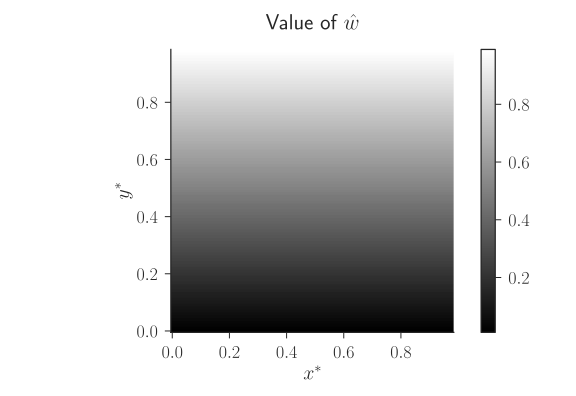
\includegraphics[width=\textwidth]{w-hat-empirical-01-marginal}
\caption{
    Estimates for $\hat{w}$ when computing $(\hat{x}, \hat{y}, \hat{w})$ using basin-hopping \citep{Wales1997} optimizing the classical marginal likelihood \eqref{eq:marginal_likelihood} (rather than a joint optimization procedure).
}
\label{fig:bl-general-marginal}
\end{figure}

\begin{figure}
\centering
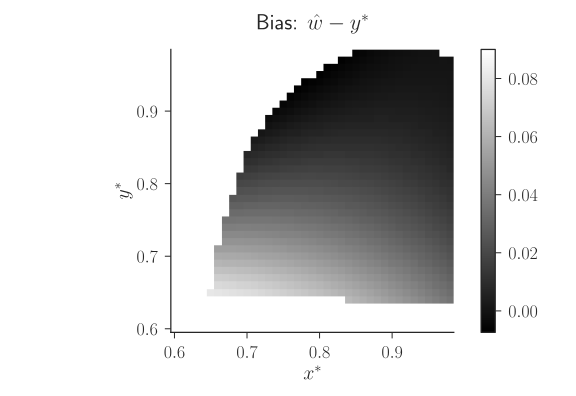
\includegraphics[width=\textwidth]{w-hat-empirical-01-bias}
\caption{
    Estimates for $\hat{w}-y^*$ when computing $(\hat{x}, \hat{y}, \hat{w})$ using basin-hopping \citep{Wales1997} optimizing \eqref{eq:profile_likelihood}.
    Plot focuses on $0.6 < x^*, y^* < 1$ where $\hat{w}$ is estimated to be a value different from 1.
    We do not compute the bias for the white region where $\hat{w}=1$ to preserve a useful scale for the rest of the plot.
}
\label{fig:bl-general-bias}
\end{figure}

